% !TeX root = ../tesis.tex

\chapter{Respuesta óptica de una monocapa desordenada de nanopartículas esféricas}
\label{chapter:Resultados}
\vspace*{5em}

Para calcular la reflectancia $R$ y transmistancia $T$  de una monocapa de nanopartículas (NPs) esféricas inmersa en un medio dieléctrico, denominado matriz, y soportada sobre un sustrato dieléctrico, se emplea el modelo de esparcimiento coherente (Coherent Scattering Model, CSM) \cite{reyes2018analytical,garcia2012multiple}. El CSM proporciona expresiones analíticas sencillas para los coeficientes de amplitud de reflexión $r$ y de transmisión $t$ de la monocapa cuando está suspendida en el espacio libre (Free Standing Monolayer, FSM) [Ecs. \eqref{eqs:rtcoh}], y para el sistema matriz-monocapa-sustrato tanto en incidencia externa [Ecs. \eqref{eqs:rtCSMext}] como interna, o bien en una configuración de reflexión total atenuada \index{Reflexión total!atenuada} (Attenuated Total Reflection, ATR) [Ecs. \eqref{eqs:rtCSMATR}]. En la primera sección de este capítulo se calcula la respuesta electromagnética (EM) de una moncapa de NPs esféricas considerando que la función dieléctrica de las NPs está dada por el modelo de Drude-Sommerfeld [Ec. \eqref{eq:Drude}],\index{Drude-Sommerfeld!modelo de!frecuencia de plasma ($\omega_p$)}\index{Drude-Sommerfeld!modelo de!constante fenomenológica de amortiguamiento ($\gamma$)} que depende de dos parámetros: la frecuencia de plasma $\omega_p$, que sintoniza las frecuencias de resonancia plasmónicas de superficie (Surface Plasmon Resonances, SPRs), y la constante fenomenológica de amortiguamiento $\gamma$, que ajusta el ancho de cada SPR. Como se muestra a continuación, la reflectancia y transmitancia de una monocapa de NPs presenta excitaciones distintas a las  SPRs de partículas individuales (Single Particle SPRs, SP-SPRs), como el \emph{modo guiado} reportado en \cite{kabashin2009plasmonic} y \cite{danilov2018ultra}, también denominado resonancia de red de superficie plasmónica (Plasmonic Surface Lattice Resonance, PSLR). Asimismo, se mostrará que la elección de $\omega_p$ y $\gamma$ evita el traslape entre las excitaciones en la monocapa y las SP-SPR, lo que facilita la identificación de cada tipo de modo. En la segunda sección se emplean las correcciones por tamaño de las funciones dieléctricas del oro y de la plata para NPs esféricas, para identificar si un modo semejante al modo guiado se encuentra presente en monocapas formadas con NPs de materiales reales, así como las  características de la monocapa para que pueda ser empleada como biosensor. Finalmente, en la tercera sección, se hace un análisis de la sensibilidad ante cambios del índice de refracción del modo excitado en la monocapa distinto de las SP-SPRs  y se compara con la sensibilidad de un biosensor comercial, que consiste en una película continua de oro donde se excita al plasmón-polaritón de superficie (Surface Plasmon Polariton, SPP), así como con arreglos nanoestructurados que se han propuesto en la literatura para el biosensado.

\section{Análisis con el modelo de Drude-Sommerfeld}
\label{section:Drude}


 En la primera subsección se analiza la reflectancia de una FSM empleando el modelo de Drude-Sommerfled con parámetros $\hbar\omega_p = 4.3$ eV y  $\hbar\gamma = 0.15$ eV [ver Fig. \ref{sfig:Drude4eV}], y se compara la respuesta EM de la monocapa con la de una partícula individual. En la segunda subsección se estudia la reflectancia de una monocapa soportada en configuración de reflexión interna atenuada, ver Fig. \ref{sfig:ATR}, empleando el modelo de Drude-Sommerfeld en un primer caso con los parámetros  $\hbar\omega_p = 4.3$ eV y  $\hbar\gamma = 0.15$ eV, y posteriormente con $\hbar\omega_p = 10$ eV y $\hbar\gamma = 0.15$ eV [ver Fig. \ref{sfig:Drude10eV}] para modificar la longitud de onda de las SP-SPRs; ulteriormente se calcula la reflectancia de la monocapa considerando  variaciones en la fracción de cubierta $\Theta$ y el radio $a$ de las NPs, parámetros que modifican la distancia mínima promedio $\langle\mathscr{D}_{min}\rangle $ entre las NPs y la cantidad de electrones libres en la monocapa. Adicionalmente, se calcula la transmitancia de la monocapa para las dos funciones dieléctricas, con $\hbar\omega_p =4.3$ eV y $\hbar\omega_p =10$ eV (con el mismo valor $\hbar\gamma=0.15$ eV), para corroborar que los modos distintos a las SP-SPRs tienen un comportamiento semejante al modo guiado o a las LSPRs reportadas en \cite{kabashin2009plasmonic} y \cite{danilov2018ultra}. 
	
	\subsection{Reflectancia de una monocapa suspendida en agua}
	\label{ssection:DrudeFSM}
	
	
Para el cálculo de la reflectancia mediante el CSM de una FSM suspendida en una matriz con $n_m=1.33$, modelando el agua en la ventana del espectro visible \cite{hale973optical}, se empleó la Ec.  \eqref{eq:R} con el coeficiente de amplitud de reflexión coherente $r_{coh}$ [Ec.  \eqref{seq:rcoh}].  En la Fig.  \ref{fig:R-FSM} se muestran los resultados de la reflectancia $R$ en función del ángulo de incidencia $\theta_i$ y tanto de la longitud de onda $\lambda$ de la onda plana incidente (escala inferior), como de la energía en unidades de $\hbar\omega = h c /\lambda$ (escala superior).  La frecuencia de plasma empleada para la función dieléctrica tipo Drude fue $\hbar\omega_p = 4. 3$ eV y la constante fenomenológica de amortiguamiento $\hbar\gamma = 0. 15$ eV (que corresponden a $288. 5$ nm  y $8,270$ nm, respectivamente). Se consideraron NPs de radio $a=30$ nm y fracciones de cubierta $\Theta$: $0. 05$, $0. 1$, $0. 2$, $0. 3$ y $0. 4$. En el renglón superior de la Fig. \ref{fig:R-FSM}, gráficas de $\mathbf{i)}$ a $\mathbf{v)}$, se muestra la reflectancia para polarización \emph{p}, mientras que en el renglón inferior  para polarización \emph{s}, \textbf{vi) -- x)}. La línea punteada vertical verde  en $\lambda \approx 658$ nm corresponde a la SP-SPR dipolar ($\ell = 1$), mientras que la línea vertical rosa punteada en $\lambda \approx 561$ nm corresponde a la excitación del modo cuadrupolar ($\ell=2$).
					
	\begin{figure}[h!]\centering
	\hspace*{-.5em}\begin{tikzpicture}[scale=1]
\node[inner sep=0pt] (graf) at (-.15,0){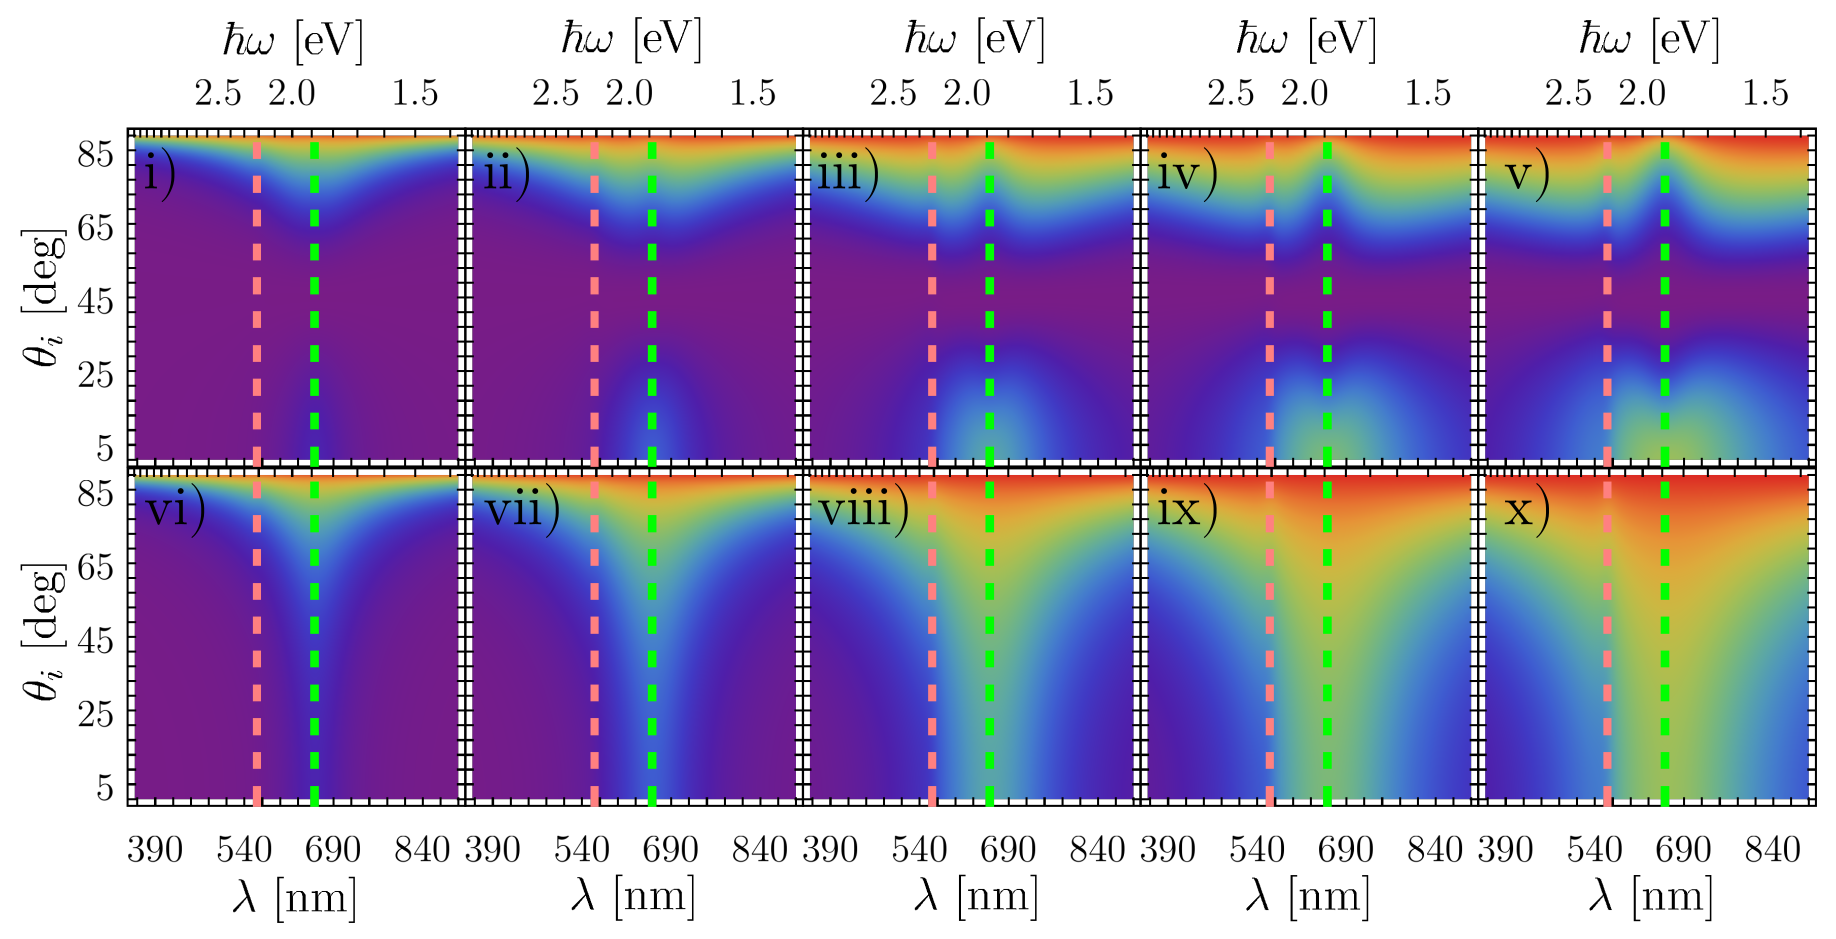
\includegraphics[scale=1]{2-Resultados/figs/4-Wp4FSMThetaVar/0-2D_Grid.png}};
\node[right, inner sep=0pt] (legend) at (7.1,.075) {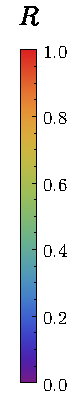
\includegraphics[scale=1, trim={00 -15 00 00}, clip]{2-Resultados/figs/0-RBar_v}};

\def\y{4.2}
	\node at(-5.2,\y){\normalsize $\Theta = 0.05 $};
	\node at(-2.4,\y){\normalsize $\Theta = 0.1 $};
	\node at(0.4,\y) {\normalsize $\Theta = 0.2$};
	\node at(3.2,\y) {\normalsize $\Theta = 0.3 $};
	\node at(6.0,\y) {\normalsize $\Theta = 0.4 $};

\def\xR{6.8}
\def\yR{2.3}	
	\node at(\xR,\yR){$R_p $};
	\node at(\xR,\yR-2.8){$R_s$};
	
\end{tikzpicture}\vspace*{-.75em}
	\caption{Gráficas de la reflectancia para una FSM como función del ángulo de incidencia $\theta_i$ y tanto de la longitud de onda $\lambda$ de la onda plana incidente (escala inferior) como de la energía en  unidades de $\hbar\omega$ (escala superior), para una función dieléctrica tipo Drude con $\hbar\omega_p=4. 3$ eV  y  $\hbar\gamma=0. 15$ eV.  Las gráficas   en el renglón superior [\textbf{i)--v)}]  muestran los resultados de la reflectancia para  polarización \emph{p} y las del renglón inferior  [\textbf{i)--v)}] para polarización  \emph{s}, donde se consideraron NPs de radio $a=30$ nm y distintas fracciones de cubierta $\Theta$: $0. 05$, $0. 1$, $0. 2$, $0. 3$ y $0. 4$. Las líneas verticales punteadas verdes y rosas corresponden a las SP-SPRs dipolar ($658$ nm) y cuadrupolar ($561$ nm), respectivamente.}	\label{fig:R-FSM}	
	\end{figure}		
					
La reflectancia para polarización \emph{p} [Fig. \ref{fig:R-FSM} \textbf{i)--v)}] es cero para el ángulo de Brewster $\theta_B = 45^\circ$ y para regiones alejadas de las SP-SPRs (líneas punteadas verticales verde y rosa). En la gráfica \textbf{v)}, $\Theta=0.4$,  se observa a $658$ nm (escala inferior) y en el intervalo $50^\circ<\theta_i<80^\circ$ que $R\approx 0$. Sin embargo, conforme el valor de $\lambda$ se aleja de $658$ nm, la reflectancia aumenta. La extinción de luz a $561$ nm  es menos evidente al disminuir la fracción de cubierta, como se observa al comparar las gráficas \textbf{iii)} y \textbf{iv)}; para las fracciones de cubierta $\Theta=0.05$ y $0.1$, gráficas \textbf{i)} y \textbf{ii)}, la extinción de luz a la frecuencia de la SP-SPR dipolar  ya no es apreciable. En contraparte, para polarización \emph{s} [Fig. \ref{fig:R-FSM} \textbf{vi)--x)}] la reflectancia es distinta de cero para todo ángulo de incidencia a las frecuencias de las SP-SPRs. 

Para comparar la respuesta EM de una FSM al variar la fracción de cubierta, se grafica en la Fig. \ref{fig:FSM-Cuts} cortes de la reflectancia mostrada en la Fig. \ref{fig:R-FSM}, para ambas polarizaciones: $R_p$ en la Fig. \ref{sfig:FSM-cutp} y  $R_s$ Fig. \ref{sfig:FSM-cuts}. Se grafican los cortes de la reflectancia a $\theta_i = 65^\circ$, pues a este ángulo se extingue la luz reflejada alrededor de la SP-SPR dipolar para polarización \emph{p} y para fracciones de cubierta $\Theta\geq 0.1$. En la Fig. \ref{sfig:FSM-cutp}, para la polarización \emph{p}, se presenta un mínimo en la reflectancia alrededor de $658$ nm para fracciones de cubierta mayores a $\Theta = 0.05$, los cuales son más pronunciados conforme aumenta la fracción de cubierta. Sin embargo, para $\Theta=0.05$ se observa un máximo en lugar de un mínimo. Para polarización \emph{s}, Fig. \ref{sfig:FSM-cuts}, se presenta un máximo en la reflectancia a $658$ nm para todos los valores de $\Theta$. Para ambas polarizaciones y a las fracciones de cubierta mayores, $\Theta = 0.3$ y $\Theta = 0.4$,  se observa un  mínimo en la reflectancia alrededor de $561$ nm  lo que corresponde a la SP-SPR cuadrupolar.

		\begin{figure}[h!]\centering\hspace*{-1.5em}
	\begin{subfigure}{.01\linewidth}\caption{}\label{sfig:FSM-cutp}\vspace{4.75cm}\end{subfigure}
	\begin{subfigure}{.45\linewidth}\hspace*{-2em}
	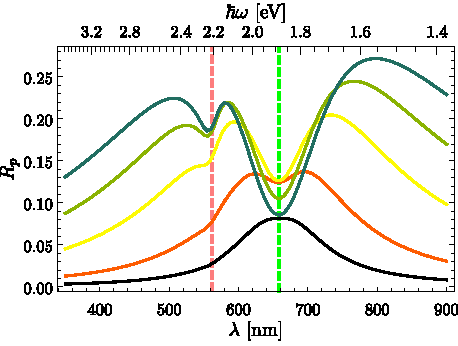
\includegraphics[scale=.98]{2-Resultados/figs/4-Wp4FSMThetaVar/cut_angle_65_p.pdf}\end{subfigure}
	\begin{subfigure}{.01\linewidth}\caption{}\label{sfig:FSM-cuts}\vspace{4.75cm}\end{subfigure}\hspace*{-1.em}
	\begin{subfigure}{.45\linewidth}\centering
	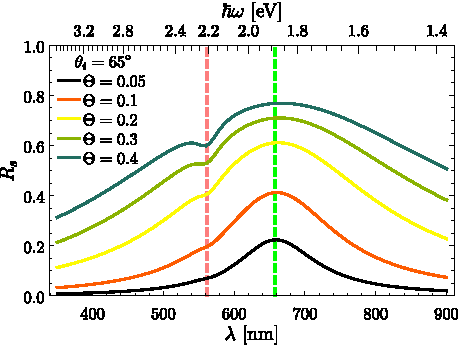
\includegraphics[scale=.98 ]{2-Resultados/figs/4-Wp4FSMThetaVar/cut_angle_65_s.pdf}\end{subfigure}\vspace*{-.5em}
	\caption{Cortes de la Fig. \ref{fig:R-FSM} a $\theta_i = 65^\circ$ de la reflectancia de una FSM de NPs esféricas de radio $a=30$ nm en polarización \textbf{a)} \emph{p} y \textbf{b)} \emph{s}, en función tanto de la longitud de onda $\lambda$ (escala inferior) como de la energía de la onda plana incidente en unidades de $\hbar\omega$ (escala superior). Los parámetros de la función dieléctrica tipo Drude para las NPs son $\hbar\omega_p = 4.3$ eV y $\hbar\gamma = 0.15$ eV y las fracciones de cubierta consideradas fueron $\Theta$: $0. 05$, $0. 1$, $0. 2$, $0. 3$ y $0. 4$. Las líneas verticales punteadas verdes y rosas corresponden a las SP-SPRs dipolar ($658$ nm) y cuadrupolar ($561$ nm), respectivamente.}\label{fig:FSM-Cuts}
	\end{figure}	

Al calcular la distancia mínima promedio $\langle\mathscr{D}_{min}\rangle$ entre las NPs  de $a = 30$ nm mediante la Tab. \ref{tab:meanD}, se obtiene que $\langle\mathscr{D}_{min}\rangle  = 177.8$ nm para $\Theta = 0.05$, por tanto el análisis de partícula individual es válido. Con este enfoque se entiende la presencia del máximo en la reflectancia de una monocapa  de NPs con $\Theta=0.05$ (en negro en la Fig. \ref{fig:FSM-Cuts}) a la longitud de onda de la SP-SPR dipolar como una cota mínima ya que, a $\lambda=658$ nm, la contribución del esparcimiento a la extinción de luz de cada una de las NPs que conforman la monocapa no es despreciable, como se observa en las eficiencias de extinción y de esparcimiento graficadas en la Fig. \ref{fig:QextDrude}.

En las Figs. \ref{fig:R-FSM} y \ref{fig:FSM-Cuts} se mostró la respuesta EM de una monocapa de NPs suspendida en un medio con $n_m=1.33$ al interactuar con una onda plana monocromática. En la presencia de un sustrato que soporte la monocapa, con índice de refracción $n_s$, es posible considerar una iluminación en configuración de incidencia externa\index{Incidencia!externa} o interna, seg\'un sea el medio de incidencia de la onda plana. Para incidencia externa, a todo ángulo de incidencia,  una onda plana iluminará a las NPs de la monocapa por lo que, respecto al caso de la FSM, la posición de los máximos y mínimos de la reflectancia no cambiarán y los valores de $R$ presentarán un decremento, debido al sustrato que disminuye el contraste entre el índice de refracción de las NPs en la monocapa y el medio de transmisión. Por otro lado, para el caso de incidencia interna y ángulos mayores al ángulo crítico $\theta_c = \arcsin(n_m/n_s)$, las NPs en la monocapa serán iluminadas por ondas evanescentes,\index{Onda!evanescente} por tratarse de una configuración ATR\index{Incidencia!interna}, por lo que es posible  observar cambios en la respuesta EM de la monocapa, como sucede  cuando se tiene una placa continua y se excitan plasmones polaritones de superficie.

	\subsection{Reflectancia y transmitancia de una monocapa soportada sobre un sustrato en configuración de reflexión total atenuada}
	\label{ssection:DrudeATR}

La respuesta EM de una monocapa de NPs embebida en una matriz con índice de refracción $n_m$ y soportada por un sustrato con índice de refracción $n_s$, se calcula al emplear la Ec.  \eqref{eq:R} con el coeficiente de amplitud de reflexión $r$ de la Ec.  \eqref{seq:rCSMATR}. Para comparar los resultados de la reflectancia de una FSM y una monocapa soportada por un sustrato e iluminada en configuración ATR, se emplean los parámetros utilizados en los cálculos de las Figs. \ref{fig:R-FSM} y \ref{fig:FSM-Cuts} ($n_m=1.33$, $a=30$ nm, $\hbar\omega_p=4.3$ eV y  $\hbar\gamma = 0.15$ eV) considerando un sustrato con índice de refracción $n_s=1.5$, modelando un vidrio BK7 cuyo índice de refracción es $1.50\pm 0.05$ en un intervalo de longitudes de onda entre $334.1$ nm y $2,325.4$ nm \cite{schott2019datasheet}. En la Fig.  \ref{fig:R-ATR4} se presentan los resultados de la reflectancia $R$ en función del ángulo de incidencia $\theta_i$ y tanto de la longitud de onda $\lambda$ (escala inferior) como de la energía $\hbar\omega$ (escala superior)  de la onda plana incidente. Las gráficas \textbf{i) -- v}) en la Fig. \ref{fig:R-ATR4}  corresponden a la polarización \emph{p}, mientras que las gráficas \textbf{vi) -- x)} a polarización \emph{s}. Al igual que para la FSM, se consideraron los casos para la fracción de cubierta $\Theta = 0.05,\,0.1,\,0.2,\,0.3$ y $0.4$. Las SP-SPRs corresponden a la línea vertical verde punteada en $\lambda \approx 658$ nm para el modo dipolar y la línea vertical rosa punteada en  $\lambda \approx 561$ nm para el modo cuadrupolar. Adicionalmente, los puntos amarillos en la Fig. \ref{fig:R-ATR4} corresponden a los mínimos en $R$ para ángulos mayores al ángulo crítico entre el sustrato y la matriz ($\theta_c\approx 62.5^\circ$), y longitudes de onda mayores a la SP-SPR dipolar.

	\begin{figure}[h!]\centering
\hspace*{-.5em}\begin{tikzpicture}[scale=1]
\node[inner sep=0pt] (graf) at (-.15,0){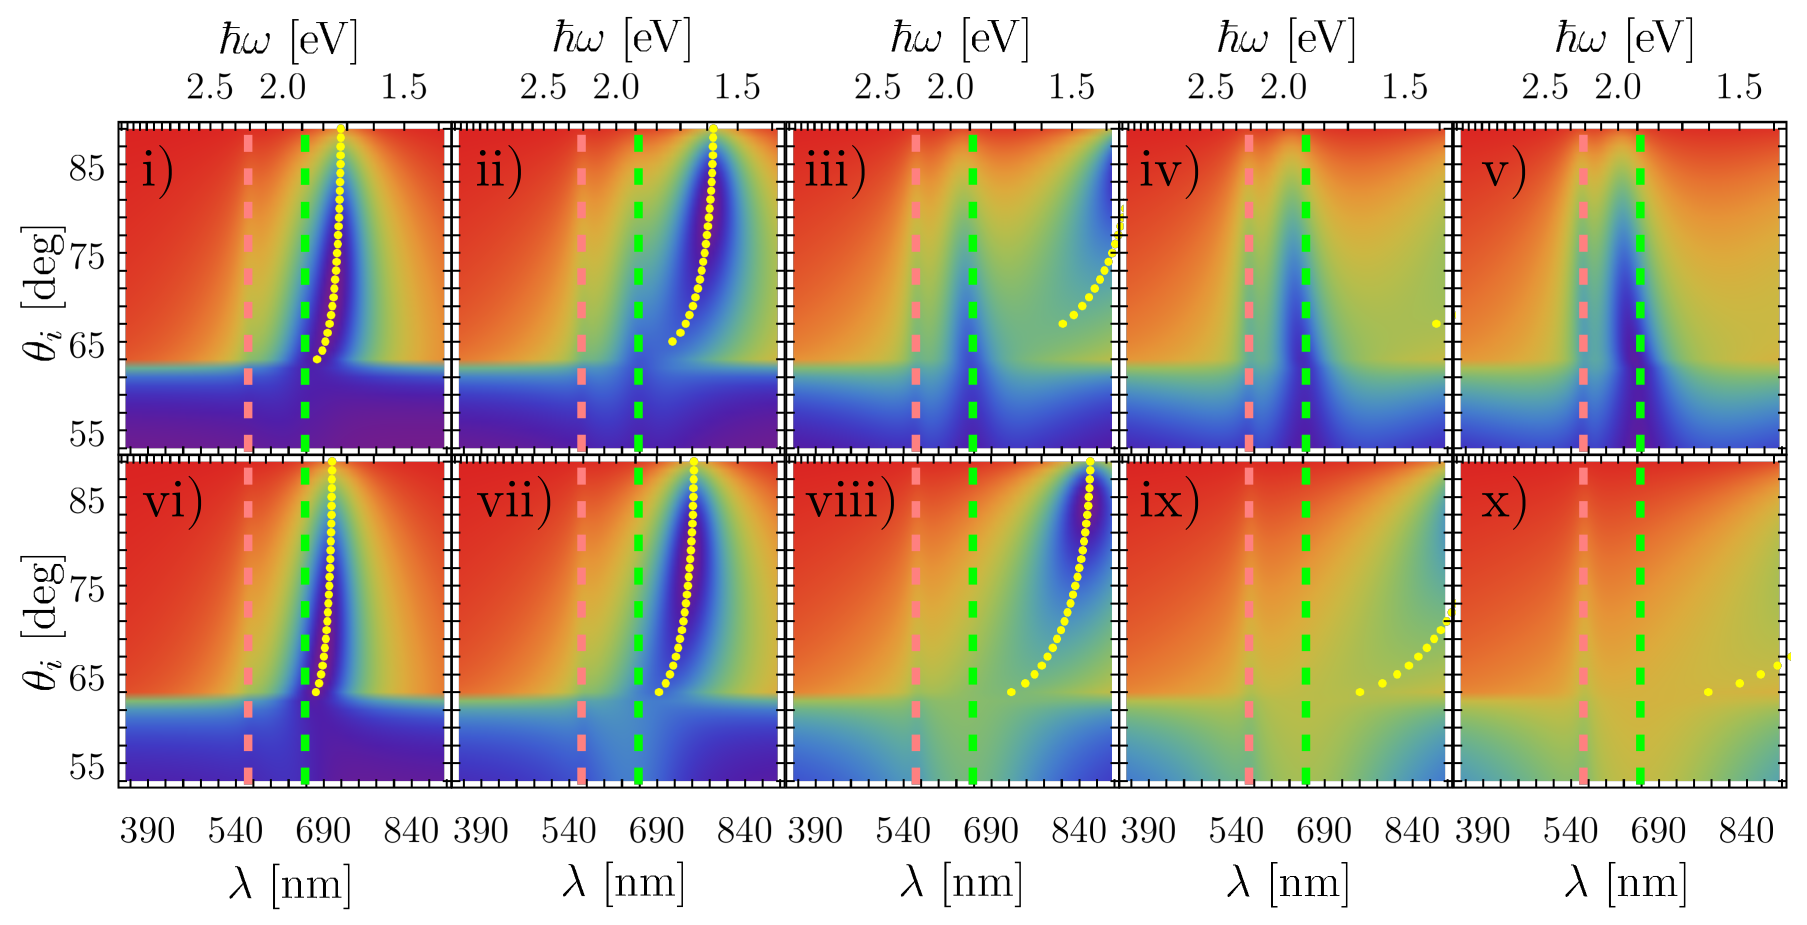
\includegraphics[scale=1]{2-Resultados/figs/1-Wp4ThetaVar/0-2D_Grid}};
\node[right, inner sep=0pt] (legend) at (7.1,.075) {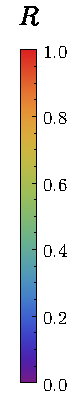
\includegraphics[scale=1, trim={00 -15 00 00}, clip]{2-Resultados/figs/0-RBar_v}};

\def\y{4.2}
	\node at(-5.2,\y){\normalsize $\Theta = 0.05 $};
	\node at(-2.4,\y){\normalsize $\Theta = 0.1 $};
	\node at(0.4,\y) {\normalsize $\Theta = 0.2$};
	\node at(3.2,\y) {\normalsize $\Theta = 0.3 $};
	\node at(6.0,\y) {\normalsize $\Theta = 0.4 $};

\def\xR{6.8}
\def\yR{2.3}	
	\node at(\xR,\yR){$R_p $};
	\node at(\xR,\yR-2.8){$R_s$};
\end{tikzpicture}\vspace*{-.5em}
	\caption{Gráficas de la reflectancia en configuración ATR de una monocapa como función del ángulo de incidencia $\theta_i$ y de la longitud de onda $\lambda$ (escala inferior) así como de la energía de la onda plana incidente en unidades de $\hbar\omega$ (escala superior), para una función dieléctrica tipo Drude con $\hbar\omega_p=4. 3$ eV  y  $\hbar\gamma=0. 15$ eV.  Las gráficas   en el renglón superior [\textbf{i)--v)}]  muestran los resultados de la reflectancia para  polarización \emph{p} y las del renglón inferior  [\textbf{vi)}--\textbf{x)}] para polarización  \emph{s}, donde se consideraron NPs de radio $a=30$ nm y distintas fracciones de cubierta $\Theta$: $0. 05$, $0. 1$, $0. 2$, $0. 3$ y $0. 4$. Las líneas verticales punteadas verdes y rosas corresponden a las SP-SPRs dipolar ($658$ nm) y cuadrupolar ($561$ nm), respectivamente. Los puntos amarillos corresponden a los mínimos en $R$ para ángulos mayores a $\theta_c\approx 62.5^\circ$ y longitudes de onda mayores a la SP-SPRs dipolar.}	\label{fig:R-ATR4}	
	\end{figure}	

En la Fig.  \ref{fig:R-ATR4} se observa que $R\approx 1$ para ángulos mayores al ángulo crítico, $\theta_c \approx 62.5^\circ$, excepto en dos regiones: a longitudes de onda correspondientes a las SP-SPRs (líneas punteadas verticales) y en una región a longitudes de onda mayores a la SP-SPR dipolar (puntos amarillos). El decremento en la reflectancia después del ángulo crítico alrededor de la SP-SPR cuadrupolar ($561$ nm) es resultado de la extinción de luz debido a la presencia de las NPs y es apreciable tanto para polarización \emph{p} como para \emph{s}, siendo más evidente para las fracciones de cubierta mayores. La respuesta óptica de la monocapa a $658$ nm (SP-SPR dipolar) es distinta para cada polarización. Mientras que en polarización \emph{p}, gráficas \textbf{i)}--\textbf{v)}, la SP-SPR dipolar se aprecia para todos los valores de $\Theta$ considerados, para polarización \emph{s}, gráficas \textbf{vi)}--\textbf{x)},  sólo se aprecia cuando $\Theta$ toma valores cercanos a cero, lo cual puede ser el traslape con la excitación distinta a las SP-SPRs que se observa en la Fig. \ref{fig:R-ATR4} (puntos amarillos).

Adicional a la región cercana a las SP-SPRs, se observan mínimos en la reflectancia para ángulos de incidencia mayores al ángulo crítico y para longitudes de onda mayores a la SP-SPR dipolar, los cuales están  representados por los puntos amarillos en la Fig. \ref{fig:R-ATR4}. Dado que los puntos amarillos corresponden a una excitación que ocurre a energías  menores en comparación a las SP-SPRs, ésta no puede ser plasmónica de partícula individual,  por lo que se especula que se debe a una respuesta plasmónica colectiva como el \emph{modo guiado} o la resonancia de red de superficie plasmónica (Plasmonic Surface Lattice Resonance, PSLR) reportada en \cite{kabashin2009plasmonic} y \cite{danilov2018ultra}. Al analizar las gráficas en la  Fig.  \ref{fig:R-ATR4} se observa que el supuesto modo plasmónico colectivo se corre al rojo  conforme aumenta la fracción de cubierta $\Theta$ y que se traslapa con la SP-SPR dipolar cuando $\Theta$ toma valores cercanos a cero, lo cual es más evidente al considerar polarización \emph{p} que \emph{s}.

Dado que la supuesta excitación colectiva presenta un mínimo en la reflectancia  alrededor de $\theta_i = 75^\circ$ para los casos de fracción de cubierta analizados en la Fig.  \ref{fig:R-ATR4}, se grafican cortes de la reflectancia a este ángulo en la Fig. \ref{fig:R-ATR4-Cuts}, en donde las líneas punteadas verticales corresponden a las longitudes de onda de las SP-SPRs (verde para la excitación dipolar y rosa para la cuadrupolar). En polarización \emph{p}, Fig. \ref{sfig:R-ATR4-cutp} la excitación de la monocapa para todos los valores de $\Theta$ alrededor de $\lambda \approx 561$ nm coincide con la SP-SPR cuadrupolar y la reflectancia disminuye conforme la fracción de cubierta crece, por lo que se relaciona con la cantidad de NPs presentes en la monocapa; para polarización \emph{s}, Fig. \ref{sfig:R-ATR4-cuts}, el mínimo en la reflectancia en la SP-SPR cuadrupolar se define mejor conforme aumenta $\Theta$ a pesar de que $R_s\approx 0.8$ para todos los valores de $\Theta$ considerados. Por otra parte, la excitación dipolar de partícula individual ($658$ nm) no se aprecia para todos los casos estudiados en la Fig. \ref{fig:R-ATR4-Cuts} y sólo coincide con un mínimo en la reflectancia para polarización \emph{p} cuando $\Theta=0.1$ nm (línea naranja), mientras que para $\Theta \geq 0.2$ se presenta un corrimiento al azul de la SP-SPR dipolar, debido a la interacción entre las NPs de la monocapa. Para $\Theta=0.05$ en polarización \emph{p} (línea sólida negra) no se observa un mínimo al valor de $\lambda$ de la SP-SPR dipolar sino a $\lambda\approx 715$ nm, asociado al supuesto modo plasmónico colectivo de la monocapa ya que a esta longitud de onda la reflectancia toma valores cercanos a cero y este comportamiento no se observa para los corrimientos al azul de la SP-SPR dipolar. Para el caso de polarización \emph{s}, no se aprecian corrimientos al azul de la SP-SPR dipolar, sino sólo se aprecia el supuesto modo plasmónico colectivo a $\lambda>658$ nm.

\begin{figure}[h!]\centering\hspace*{-1.5em}
	\begin{subfigure}{.01\linewidth}\caption{}\label{sfig:R-ATR4-cutp}\vspace{4.75cm}\end{subfigure}
	\begin{subfigure}{.45\linewidth}\hspace*{-1.5em}
	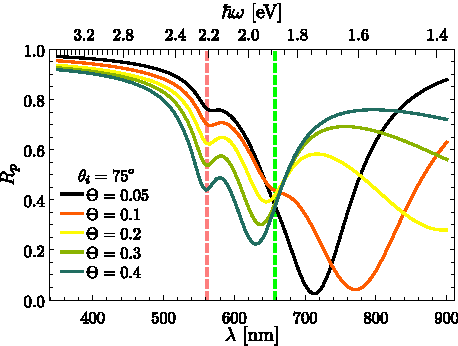
\includegraphics[scale=.98]{2-Resultados/figs/1-Wp4ThetaVar/cut_angle_75_p.pdf}\end{subfigure}
	\begin{subfigure}{.01\linewidth}\caption{}\label{sfig:R-ATR4-cuts}\vspace{4.75cm}\end{subfigure}\hspace*{-1.em}
	\begin{subfigure}{.45\linewidth}\centering
	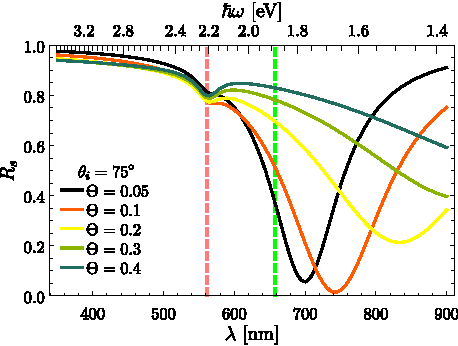
\includegraphics[scale=.98 ]{2-Resultados/figs/1-Wp4ThetaVar/cut_angle_75_s.pdf}\end{subfigure}\vspace*{-.5em}
	\caption{
Cortes de la reflectancia mostrada en la Fig. \ref{fig:R-ATR4} a $\theta_i = 75^\circ$ para una monocapa iluminada en configuración ATR de NPs esféricas de radio $a=30$ nm en polarización \textbf{a)} \emph{p} y \textbf{b)} \emph{s} como función de la longitud de onda $\lambda$ (escala inferior) y de la energía $\hbar\omega$ (escala superior). Los parámetros de la función dieléctrica tipo Drude para las NPs son $\hbar\omega_p = 4.3$ eV y $\hbar\gamma = 0.15$ eV y las fracciones de cubierta consideradas fueron $\Theta$: $0. 05$, $0. 1$, $0. 2$, $0. 3$ y $0. 4$. Las líneas verticales punteadas verdes y rosas corresponden a las SP-SPRs dipolar ($658$ nm) y cuadrupolar ($561$ nm), respectivamente. }\label{fig:R-ATR4-Cuts}
	\end{figure}

Los mínimos de la reflectancia a $\lambda>650$ nm en la Fig. \ref{fig:R-ATR4-Cuts}, que corresponden al supuesto modo plasmónico colectivo, presentan un corrimiento al rojo conforme la fracción de cubierta de la monocapa aumenta  para ambas polarizaciones, contrario al comportamiento observado en las excitaciones plasmónicas de partícula individual de la monocapa observadas en la Fig. \ref{sfig:R-ATR4-cutp}, entre $561$ nm y $658$ nm. Otra diferencia entre las excitaciones en $\lambda$ mayores a las SP-SPRs y los corrimientos al azul de éstas, es que el decremento en el valor de $R$ no es monótono, sino que se aprecia un máximo a fracciones de cubierta intermedias (ver Fig. \ref{fig:R-ATR4-Cuts}, casos $\Theta=0.05$, $0.1$ y $0.2$). El corrimiento al rojo del supuesto modo plasmónico colectivo es mayor para  polarización \emph{p} que para \emph{s}, como se observa en la Fig. \ref{fig:R-ATR4-Cuts}. Por ejemplo, para $\Theta=0.1$ (línea naranja sólida), el mínimo en $R$ se localiza a $765$ nm para \emph{p} y  a $740$ nm para \emph{s}. Por lo anterior, los mínimos en $R_p$ y $R_s$ localizados a longitudes de onda mayores a la de los modos plasmónicos de partícula individual no son corrimientos de las excitaciones multipolares de una partícula aislada, sino una respuesta colectiva de las NPs en la monocapa. 

En la Fig. \ref{fig:R-ATR4-Cuts}, para $\Theta = 0.3$ y $0.4$ a ambas polarizaciones, el supuesto modo plasmónico colectivo se separa de la SP-SPRs dipolar (línea punteada vertical verde) a longitudes mayores a $900$ nm ---región en donde el agua presenta absorción---, por lo que 
no son apreciables en la Fig. \ref{fig:R-ATR4-Cuts}. Sin embargo, al elegir valores de $\Theta$ entre $0.05$ y $0.2$, es posible sintonizar la resonancia del supuesto modo plasmónico colectivo entre $695$ nm y $830$ nm para polarización \emph{p}, o bien, entre $715$ nm y $815$ nm para polarización \emph{s}. 

Para caracterizar el supuesto modo plasmónico colectivo se repitieron los cálculos de la reflectancia modificando la frecuencia de plasma en el modelo de Drude, que caracteriza la respuesta EM de las NPs y modifica la posición de las SP-SPRs. Los resultados de la reflectancia de un sistema monocapa con los parámetros empleados en la Fig. \ref{fig:R-ATR4}, pero con $\hbar\omega_p = 10$ eV, se muestran en la Fig. \ref{fig:R-ATR10}. Dado que $\omega_p\propto\sqrt{n_v}$, con $n_v$ la densidad volumétrica electrónica [Ec. \eqref{eq:wp}], para $\hbar\omega_p = 10$ eV se considera un mayor número de electrones libres en comparación con $\hbar\omega_p=4.3$ eV, y por tanto se espera que las resonancias, tanto las SP-SPRs como la del supuesto modo plasmónico colectivo, sean más intensas. En la Fig. \ref{fig:R-ATR10} las líneas verticales punteadas verde y rosa en $342$ nm y $262$ nm corresponden nuevamente a las SP-SPRs dipolar y cuadrupolar (que se corren al azul respecto a las SP-SPR obtenidas con $\hbar\omega_p=4.3$ eV), respectivamente, mientras que los puntos amarillos corresponden a los mínimos en la reflectancia asociados al supuesto modo plasmónico colectivo.
				
\begin{figure}[h!]\centering
\hspace*{-.5em}\begin{tikzpicture}[scale=1]
\node[inner sep=0pt] (graf) at (-.15,0){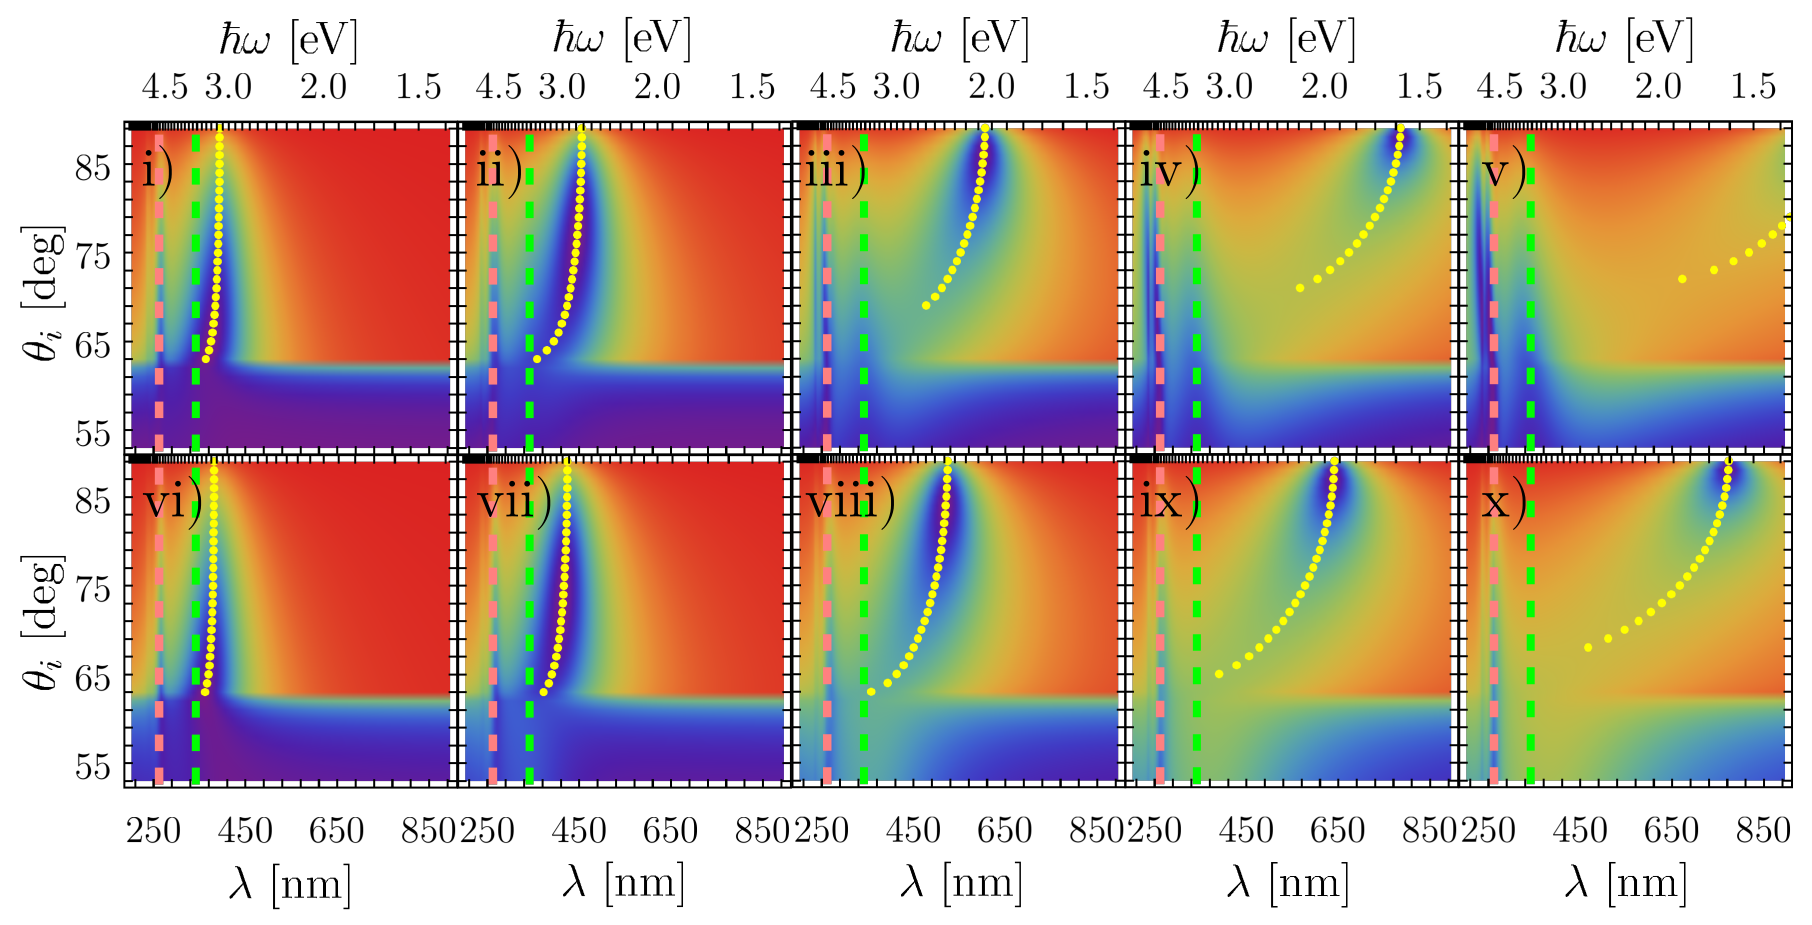
\includegraphics[scale=1]{2-Resultados/figs/2-Wp10ThetaVar/0-2D_Grid}};
\node[right, inner sep=0pt] (legend) at (7.1,.085) {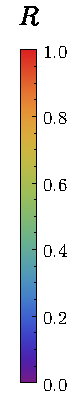
\includegraphics[scale=1, trim={00 -15 00 00}, clip]{2-Resultados/figs/0-RBar_v}};

\def\y{4.2}
	\node at(-5.2,\y){\normalsize $\Theta = 0.05 $};
	\node at(-2.4,\y){\normalsize $\Theta = 0.1 $};
	\node at(0.4,\y) {\normalsize $\Theta = 0.2$};
	\node at(3.2,\y) {\normalsize $\Theta = 0.3 $};
	\node at(6.0,\y) {\normalsize $\Theta = 0.4 $};

\def\xR{7}
\def\yR{2.5}	
	\node at(\xR,\yR){$R_p $};
	\node at(\xR-.75,\yR-2.8){$R_s$};
\end{tikzpicture}\vspace*{-.5em}
	\caption{Gráficas de la reflectancia en configuración ATR de una monocapa como función del ángulo de incidencia $\theta_i$ y de la longitud de onda $\lambda$ (escala inferior), así como de la energía de la onda plana incidente en unidades de $\hbar\omega$ (escala superior), para una función dieléctrica tipo Drude con $\hbar\omega_p=10$ eV  y  $\hbar\gamma=0. 15$ eV.  Las gráficas   en el renglón superior [\textbf{i)--v)}] muestran los resultados  para  polarización \emph{p} y las del renglón inferior  [\textbf{vi)}--\textbf{x)}] para polarización  \emph{s}, donde se consideraron NPs de radio $a=30$ nm y distintas fracciones de cubierta $\Theta$: $0. 05$, $0. 1$, $0. 2$, $0. 3$ y $0. 4$. Las líneas verticales punteadas verdes y rosas corresponden a las SP-SPRs dipolar ($342$ nm) y cuadrupolar ($262$ nm), respectivamente.  Los puntos amarillos corresponden a los mínimos en $R$ para ángulos mayores a $\theta_c\approx 62.5^\circ$ y longitudes de onda mayores a la SP-SPRs dipolar. }	\label{fig:R-ATR10}	
	\end{figure}		
	
En las gráficas mostradas en la Fig. \ref{fig:R-ATR10} ($\hbar\omega_p = 10$ eV), como es de esperarse, se aprecian características semejantes a las observadas en la Fig. \ref{fig:R-ATR4}, en las que se empleó $\hbar\omega_p = 4.3$ eV. La excitación de la SP-SPR dipolar (líneas verticales punteadas verdes) sólo es apreciable para polarización \emph{p} (para todas las fracciones de cubierta consideradas). En ambas polarizaciones, la reflectancia, considerando $\theta_i>\theta_c$, disminuye para valores de $\lambda$ cercanos a la SP-SPR cuadrupolar (líneas verticales punteadas rosas), así como a longitudes de onda mayores a la SP-SPR dipolar, es decir, en la supuesta excitación colectiva  (puntos amarillos); de igual forma, el corrimeinto al rojo de la supuesta excitación colectiva respecto a la SP-SPR dipolar es mayor para polarización \emph{p} que para \emph{s}.  Asimismo, al modificar el parámetro $\hbar\omega_p$ de $4.3$ eV a $10$ eV se sintonizó la supuesta excitación colectiva a longitudes de onda menores, por ejemplo, para $\Theta = 0.3$, para todo ángulo de incidencia, la supuesta excitación colectiva se localiza a $\lambda<900$ nm para $\hbar\omega_p=10$ eV, mientras que para $\hbar\omega_p=4.3$ eV el modo colectivo ya no se apreciaba en el espectro visible (ver gráficas \textbf{iv)} y \textbf{ix)} de las Figs. \ref{fig:R-ATR4} y \ref{fig:R-ATR10}).

\begin{figure}[b!]\centering\hspace*{-1.5em}
	\begin{subfigure}{.01\linewidth}\caption{}\label{sfig:R-ATR10-cutp}\vspace{4.75cm}\end{subfigure}
	\begin{subfigure}{.45\linewidth}\hspace*{-1.5em}
	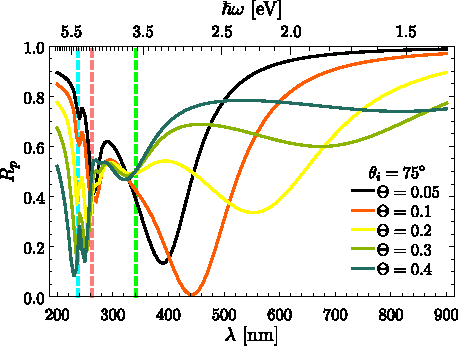
\includegraphics[scale=.98]{2-Resultados/figs/2-Wp10ThetaVar/cut_angle_75_p.pdf}\end{subfigure}
	\begin{subfigure}{.01\linewidth}\caption{}\label{sfig:R-ATR10-cuts}\vspace{4.75cm}\end{subfigure}\hspace*{-1.em}
	\begin{subfigure}{.45\linewidth}\centering
	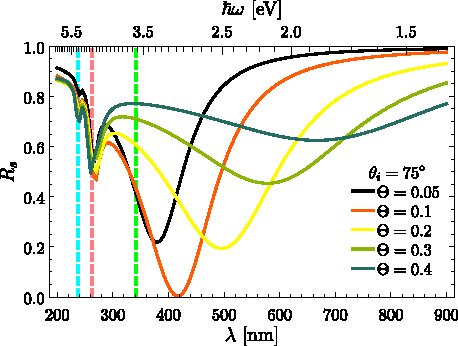
\includegraphics[scale=.98 ]{2-Resultados/figs/2-Wp10ThetaVar/cut_angle_75_s.pdf}\end{subfigure}\vspace*{-.5em}
	\caption{Cortes de la reflectancia mostrada en la Fig. \ref{fig:R-ATR10} a $\theta_i = 75^\circ$ para una monocapa iluminada en configuración ATR de NPs esféricas de radio $a=30$ nm en polarización \textbf{a)} \emph{p} y \textbf{b)} \emph{s} como función de la longitud de onda $\lambda$ (escala inferior) y de la energía en unidades de $\hbar\omega$ (escala superior). Los parámetros de la función dieléctrica tipo Drude para las NPs son $\hbar\omega_p = 10$ eV y $\hbar\gamma = 0.15$ eV y las fracciones de cubierta consideradas fueron $\Theta$: $0. 05$, $0. 1$, $0. 2$, $0. 3$ y $0. 4$. Las líneas verticales punteadas verdes, rosas y cianes corresponden a las SP-SPRs dipolar ($342$ nm), cuadrupolar ($262$ nm) y octopolar ($238$ nm), respectivamente.  }\label{fig:R-ATR10-Cuts}
	\end{figure}

Dado que la elección del parámetro $\omega_p$ sintoniza a las SP-SPRs y al supuesto modo plasmónico colectivo, la separación entre estos puede modificarse. Para comparar con el caso de $\hbar\omega_p=4.3$ eV (Fig. \ref{fig:R-ATR4-Cuts}), se grafica en la Fig. \ref{fig:R-ATR10-Cuts} cortes de la reflectancia graficada en la Fig. \ref{fig:R-ATR10}, donde se emplea $\hbar\omega_p = 10$ eV, a $\theta_i = 75^\circ$ para ambas polarizaciones,  Fig. \ref{sfig:R-ATR10-cutp} para \emph{p} y Fig. \ref{sfig:R-ATR10-cuts} para \emph{s}, en  función de la longitud de onda de la onda plana incidente, para una monocapa de NPs de radio $a= 30$ nm  y fracciones de cubierta consideradas en la Fig. \ref{fig:R-ATR10}; las líneas punteadas verde y rosa  corresponden a las SP-SPRs dipolar y cuadrupolar, respectivamente. Para ambas polarizaciones y para todas las fracciones de cubierta, se presenta una excitación a la longitud de onda correspondiente a la SP-SPR octopolar en $\lambda=240$ nm (línea punteada vertical cian), la cual se corre al azul para ambas polarizaciones, al igual que  la SP-SPR cuadrupolar alrededor de $262$ nm (línea punteada vertical rosa). De forma semejante a los resultados obtenidos con $\hbar\omega_p = 4.3$ eV (Fig. \ref{fig:R-ATR4-Cuts}), la reflectancia de la monocapa considerando $\hbar\omega_p=10$ eV y $\theta_i=75^\circ$ (Fig. \ref{fig:R-ATR10-Cuts}) se presenta un corrimiento al azul de la SP-SPR dipolar (línea punteada vertical verde) para $\Theta\geq 0.2$, que aumenta conforme $\Theta$ crece. Sin embargo, para $\Theta=0.05$ y $0.1$ en polarización \emph{p}, y para todos los valores de $\Theta$ considerados para \emph{s}, la SP-SPR dipolar no se aprecia en los cálculos de la reflectancia. En su lugar, se observan mínimos  localizados a longitudes de onda mayores a $342$ nm, atribuidos al supuesto modo plasmónico colectivo.

En la Fig. \ref{fig:R-ATR10-Cuts} ($\hbar\omega_p=10$ eV), los mínimos de reflectancia a $\lambda > 342$ nm se atribuyen a una supuesta respuesta colectiva de las NPs en la monocapa. De forma análoga al caso $\hbar\omega_p = 4.3$ eV (Fig. \ref{fig:R-ATR4-Cuts}), para $\hbar\omega=10$ eV los mínimos de reflectancia se corren al rojo conforme aumenta la fracción de cubierta y su presencia es más evidente para fracciones de cubierta intermedia, siendo  $\Theta=0.1$ cuando la reflectancia en la excitación del supuesto modo plasmónico colectivo alcanza un valor mínimo. Cuando $\Theta = 0.05$ (líneas negras en la Fig. \ref{fig:R-ATR10-Cuts}) la excitación del supuesto modo plasmónico colectivo se separa de la SP-SPR dipolar  aproximadamente $40$ nm para ambas polarizaciones, mientras que para $\Theta = 0.2$ la excitación del supuesto modo plasmónico colectivo se separa de la SP-SPR dipolar  $210$ nm y $160$ nm para polarización \emph{p} y \emph{s}, respectivamente. Es decir, que la separación entre la SP-SPR dipolar y el supuesto modo plasmónico colectivo es menor que cuando se consideró $\hbar\omega_p = 4.3$ eV en la Fig. \ref{fig:R-ATR4-Cuts} (en donde, para $\Theta=0.2$, la supuesta excitación colectiva se separó de la SP-SPR dipolar $240$ nm y $200$ nm para polarización \emph{p} y \emph{s}, respectivamente). Por otra parte, la anchura a media altura (Full Width at Half Maximum, FWHM)\index{Anchura a media altura (FWHM) ($\Gamma$)} $\Gamma$ de la supuesta excitación colectiva es mayor para $\hbar\omega_p=10$ eV en comparación a $\hbar\omega_p=4.3$ eV. Por ejemplo, para $\Theta = 0.05$ y $\hbar\omega_p = 4.3$ eV,  $\Gamma\approx 140$ nm para polarización \emph{p} y  $\Gamma\approx 120$ nm para  \emph{s} (ver Fig. \ref{fig:R-ATR4-Cuts}), mientras que para  $\hbar\omega_p = 10$ eV,  $\Gamma\approx 180$ nm para polarización \emph{p} y  $\Gamma\approx 140$ nm para  \emph{s} (ver Fig. \ref{fig:R-ATR10-Cuts}).

Ya que el supuesto modo plasmónico colectivo sufre un corrimiento al rojo al aumentar la fracción de cubierta, parámetro que modifica el volumen neto de material plasmónico ---es decir, la cantidad de electrones libres en la monocapa---, disminuyendo la distancia mínima promedio $\langle\mathscr{D}_{min}\rangle$ entre las NPs, se analizó si el comportamiento es semejante a cambios en el radio $a$ de las NPs, parámetro que también modifica la cantidad de electrones libres en la monocapa. Si  los mínimos en la reflectancia  a energías menores que la SP-SPR dipolar son sensibles al radio de las NPs, como lo son con la fracción de cubierta, se refuerza la idea de que esta excitación se debe a un efecto colectivo de los electrones libres en las NPs.
 
\begin{figure}[h!]\centering
\hspace*{-.5em}\begin{tikzpicture}[scale=1]
\node[inner sep=0pt] (graf) at (-.15,0){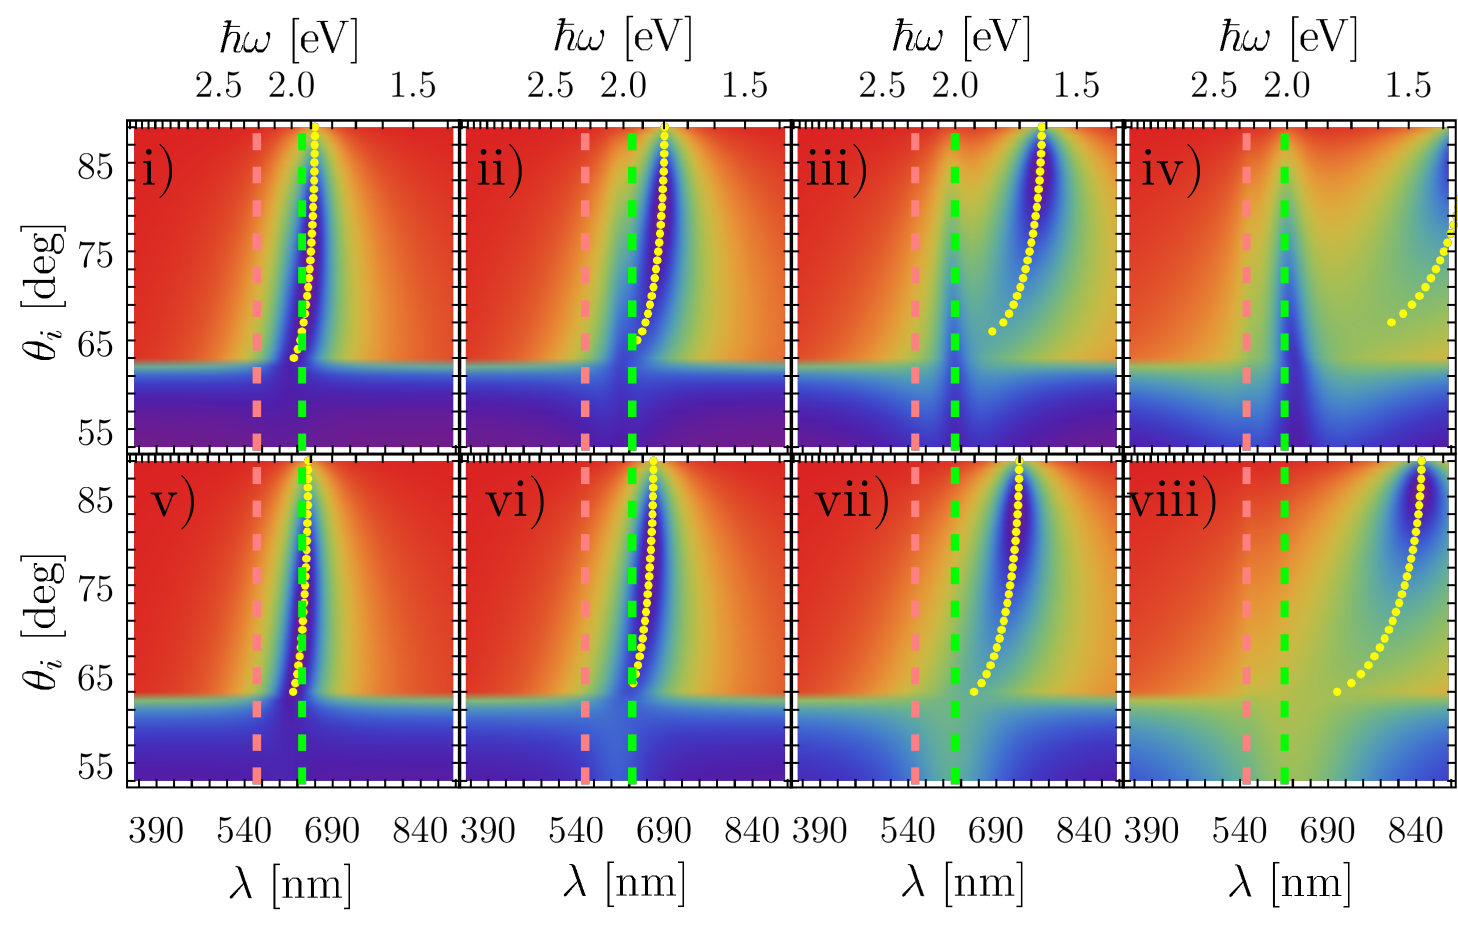
\includegraphics[scale=1]{2-Resultados/figs/3-Wp4rVar/0-2D_Grid}};
\node[right, inner sep=0pt] (legend) at (5.75,.0775) {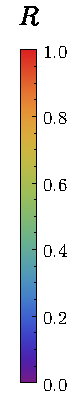
\includegraphics[scale=1, trim={00 -15 00 00}, clip]{2-Resultados/figs/0-RBar_v}};

\def\y{4.2}
	\node at(-3.85,\y){\normalsize $a = 3 $ nm};
	\node at(-1,\y){\normalsize $a = 5 $ nm};
	\node at(1.8,\y) {\normalsize $a = 10$ nm};
	\node at(4.7,\y) {\normalsize $a = 20$ nm};
%	\node at(6.0,\y) {\normalsize $\Theta = 0.4 $};

\def\xR{5.3}
\def\yR{2.5}	
	\node at(\xR,\yR){$R_p $};
	\node at(\xR,\yR-2.8){$R_s$};
\end{tikzpicture}\vspace*{-.5em}
	\caption{Gráficas de la reflectancia en configuración ATR de una monocapa como función del ángulo de incidencia $\theta_i$ y de la longitud de onda $\lambda$ (escala inferior), así como de la energía de la onda plana incidente en unidades de $\hbar\omega$ (escala superior), para una función dieléctrica tipo Drude con $\hbar\omega_p=4.3$ eV  y  $\hbar\gamma=0. 15$ eV.  Las gráficas   en el renglón superior [\textbf{i)--v)}] muestran los resultados para  polarización \emph{p} y las del renglón inferior  [\textbf{vi)}--\textbf{x)}]  para polarización  \emph{s}, donde se consideró una fracción de cubierta $\Theta = 0.3$ y  NPs de radio  $a$: $3$ nm, $5$ nm, $10$ nm y $20$ nm.  Las líneas verticales punteadas verdes y rosas corresponden a las SP-SPRs dipolar y  cuadrupolar, respectivamente.  Los puntos amarillos corresponden a los mínimos en $R$ para ángulos mayores a $\theta_c\approx 62.5^\circ$ y longitudes de onda mayores a la SP-SPRs dipolar.
}	\label{fig:R-RVar}	
	\end{figure}	

Los resultados de la reflectancia de una monocapa con $\Theta=0.3$, inmersa en un medio con índice de refracción $n_m = 1.33$ y soportada por un sustrato con índice de refracción $n_m= 1.5$, se muestran en la Fig.  \ref{fig:R-RVar}, como función del ángulo de incidencia, tanto de la longitud de onda $\lambda$ (escala inferior) como de la  energía $\hbar\omega$ (escala superior) de la onda plana incidente. Se consideraron NPs  con una respuesta EM dada por una función dieléctrica  tipo Drude [Ec. \eqref{eq:Drude}] con los parámetros $\hbar\omega_p =4.3$ eV y $\hbar\gamma=0.15$ eV, con radios $a$: $3$ nm, $5$ nm, $10$ nm y $20$ nm. La reflectancia en polarización \emph{p} se presenta en las gráficas \textbf{i)--iv)}, mientras que en \emph{s}, en las gráficas \textbf{v)--viii)}. Las SP-SPRs dipolar y cuadrupolar corresponden a las líneas punteadas verde y rosa, respectivamente. Para $a = 3$ nm y $5$ nm la excitación dipolar se localiza en $\lambda\approx 615$ nm, para el radio  $a = 10$ nm en $\lambda\approx 620$ nm y $a=20$ nm en $\lambda\approx 635$ nm, mientras que la SP-SPR cuadrupolar se localiza en $\lambda\approx 551$ nm para $a\leq 10$ nm y para el caso  $a=20$ nm, $\lambda \approx 555$ nm.	
	
En la Fig.   \ref{fig:R-RVar} (variación del radio $a$) la respuesta EM de la monocapa es análoga a la observada en la Fig. \ref{fig:R-ATR4} (variación de $\Theta$): la reflectancia, considerando $\theta_i>\theta_c\approx 62.5^\circ$, es menor a $1$ en las SP-SPRs (líneas punteadas verticales) y en valores de $\lambda$ mayores a las de la SP-SPR dipolar (puntos amarillos). La distancia entre estas regiones aumenta al crecer el radio de las NPs, al igual que lo hacía al aumentar la fracción de cubierta, además de que también esta distancia es mayor para polarización \emph{p}, que para \emph{s}. Asimismo, la SP-SPR dipolar sólo es apreciable para polarización \emph{p} a partir de NPs con radios $a\geq 10$ nm; para \emph{s} la resonancia sólo es apreciable para ángulos menores al ángulo crítico ($\theta_c\approx 62.5^\circ$). Dado que la excitación a energías menores a las de las SP-SPRs (puntos amarillos) se modifica al aumentar el radio de las NPs, al igual que al cambiar el valor de la fracción de cubierta, esta excitación puede corresponder a un modo colectivo, ya que responde a la cantidad neta de material plasmónico ---de electrones libres--- presentes en la monocapa. Para analizar la respuesta EM de la monocapa al aumentar el radio de las NPs, y compararla con la variación en $\Theta$ en la Fig. \ref{fig:R-ATR4-Cuts},  se grafican en la Fig. \ref{fig:R-RVar-Cuts}  cortes de la reflectancia de la Fig. \ref{fig:R-RVar} a $\theta_i = 75^\circ$. La región sombreada verde entre $615$ nm y $658$ nm corresponde al intervalo en $\lambda$ donde se localizan las SP-SPRs dipolares para las NPs empleadas (con radios $3\mbox{ nm}\leq a \leq 20\mbox{ nm}$), y la región sombreada rosa entre $551$ nm y $561$ nm donde se localizan las SP-SPRs cuadrupolares.

\begin{figure}[h!]\centering\hspace*{-1.5em}
	\begin{subfigure}{.01\linewidth}\caption{}\label{sfig:R-RVar-cutp}\vspace{4.75cm}\end{subfigure}
	\begin{subfigure}{.45\linewidth}\hspace*{-1.5em}
	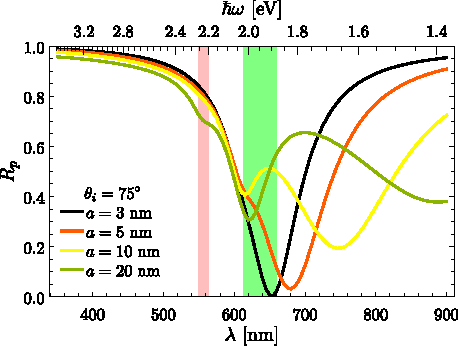
\includegraphics[scale=.98]{2-Resultados/figs/3-Wp4rVar/cut_angle_75_p.pdf}\end{subfigure}
	\begin{subfigure}{.01\linewidth}\caption{}\label{sfig:R-RVar-cuts}\vspace{4.75cm}\end{subfigure}\hspace*{-1.em}
	\begin{subfigure}{.45\linewidth}\centering
	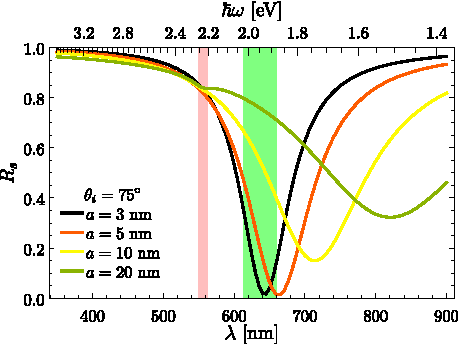
\includegraphics[scale=.98 ]{2-Resultados/figs/3-Wp4rVar/cut_angle_75_s.pdf}\end{subfigure}\vspace*{-.5em}
	\caption{Cortes de la reflectancia mostrada en la Fig. \ref{fig:R-RVar} a $\theta_i = 75^\circ$ para una monocapa iluminada en configuración ATR de NPs esféricas de fracción de cubierta $\Theta = 0.3$ en polarización \textbf{a)} \emph{p} y \textbf{b)} \emph{s} en función de la longitud de onda $\lambda$ (escala inferior) y de la energía $\hbar\omega$ (escala superior). Los parámetros de la función dieléctrica tipo Drude para las NPs son $\hbar\omega_p = 4.3$ eV y $\hbar\gamma = 0.15$ eV, y los radios  considerados fueron $a$: $3$ nm, $5$ nm, $10$ nm y $20$ nm. La SP-SPR dipolar para los tamaños de partículas utilizadas corresponde la región verde entre $615$ nm y $658$ nm, mientras que la cuadrupolar corresponde a la región rosa entre $551$ nm y $561$ nm.}\label{fig:R-RVar-Cuts}
	\end{figure}	

En los resultados de la reflectancia para polarización \emph{p}, graficados en la Fig. \ref{sfig:R-RVar-cutp}, la excitación cuadrupolar sólo es apreciable para $a=20$ nm, mientras que la SP-SPR dipolar sólo se aprecia para los radios de $10$ nm y $20$ nm (líneas amarilla y verde) a $\lambda\approx 620$ nm. Para $a=5$ nm, la reflectancia evaluada en $\lambda\approx 620$ nm no es mínima, sin embargo se presenta un cambio en la pendiente de la reflectancia; adicionalmente, en $690$ nm, la reflectancia para $a=5$ nm tiene un mínimo con $R_p<0.1$, el cual se atribuye al supuesto modo plasmónico colectivo. Para $a=3$ nm (línea negra) no se manifiesta la SP-SPR dipolar sino únicamente el mínimo correspondiente al supuesto modo plasmónico colectivo a $650$ nm, en donde $R_p\approx 0$. A partir del comportamiento de $R_p$ para $a=3$ nm y $a=5$ nm a $620$ nm, así como el corrimiento al rojo de la excitación del supuesto modo plasmónico colectivo al aumentar el radio de las NPs en la monocapa, se concluye que para NPs con radios tendiendo a cero, la supuesta excitación colectiva corresponde a la de partícula individual.
 
 Para polarización \emph{s}, Fig. \ref{sfig:R-RVar-cuts}, la respuesta cuadrupolar sólo se observa para $a = 20$ nm y, como ocurrió en casos anteriores (Figs. \ref{fig:R-ATR4-Cuts} y \ref{fig:R-ATR10-Cuts}), la SP-SPR dipolar no es apreciable. Las excitaciones a $\lambda>620$ nm en la Fig. \ref{fig:R-RVar-Cuts} siguen las tendencias observadas para el supuesto modo plasmónico colectivo: corrimiento al rojo al aumentar el valor de $a$ y $R_s\approx 0$ a las longitudes de onda del supuesto modo plasmónico colectivo. Por lo tanto, estas excitaciones se atribuyen al modo plasmónico colectivo y se corrobora que la excitación colectiva se traslapa con la SP-SPR dipolar cuando el radio de las NPs tiende a cero, tanto para polarización \emph{p} como para \emph{s}.
 
La respuesta óptica de la monocapa correspondiente al supuesto modo plasmónico colectivo presenta, a un valor de $\theta_i$ fijo (Figs. \ref{fig:R-ATR4-Cuts}, \ref{fig:R-ATR10-Cuts} y \ref{fig:R-RVar-Cuts}), tanto un ensanchamiento de la resonancia como un corrimiento al rojo, al aumentar la fracción de cubierta de la monocapa o el radio de las NPs que la conforman. El supuesto modo plasmónico colectivo también se corre al rojo al aumentar el ángulo de incidencia, como se observa en las Figs. \ref{fig:R-ATR4}, \ref{fig:R-ATR10} y \ref{fig:R-RVar}, y la reflectancia a las longitudes de onda de la supuesta excitación colectiva decrece conforme aumenta el ángulo de incidencia (para después llegar a $R=1$ a incidencia rasante, como es de esperarse), como se evidencia en los casos con $\Theta=0.3$ y $0.4$ (Figs. \ref{fig:R-ATR10} y \ref{fig:R-RVar}); otro efecto en la elección del ángulo de incidencia es que la FWHM del supuesto modo plasmónico colectivo disminuye al aumentar $\theta_i$. La SP-SPR dipolar coincide con el supuesto modo plasmónico colectivo cuando los radios de la NPs de la monocapa, o su fracción de cubierta, tienden a cero y cuando los ángulos de incidencia son cercanos al ángulo crítico $\theta_c$. Asimismo, para polarización \emph{p} la SP-SPR dipolar es apreciable en la reflectancia y distinguible del modo colectivo, mientras que para \emph{s} no se aprecia. El valor de la reflectancia a las longitudes de onda de la supuesta excitación colectiva, así como su ancho, dependen del material de las NPs. Por ejemplo, para polarización \emph{p}, considerando  $a=30$ nm, $\Theta=0.05$ y $\theta_i=75^\circ$, $\hbar\omega_p=4.3$ eV la reflectancia es mínima para $\lambda=715$ nm  [ver Fig. \ref{sfig:R-ATR4-cutp}], mientras que para $\hbar\omega_p=10$ eV es mínima para $\lambda=380$ nm [ver Fig. \ref{sfig:R-ATR10-cutp}].

El supuesto modo plasmónico colectivo se caracterizó por medio del análisis de la reflectancia de la monocapa empleando el CSM, mostrando que a ciertas longitudes de onda ---mayores que las SP-SPRs, por lo que no pueden corresponder a excitaciones de partícula individual---, $\lambda^{exc}$, la reflectancia es cercana a cero. Es decir, que la energía del haz incidente no se refleja a $\lambda^{exc}$ pero bien podría transmitirse hacia el sustrato. Por tanto, se calculó la transmitancia del sistema. 

% Dado que el supuesto modo plasmónico colectivo se presenta a energías menores que las de SP-SPRs, ésta no es una excitación plasmónica de partícula individual, de forma semejante que el \emph{modo guiado} y las PSLRs reportadas en  \cite{kabashin2009plasmonic} y \cite{danilov2018ultra}, respectivamente. Sin embargo, la PSLR tiene características de un modo guiado, es decir, que la energía transportada por esta excitación se propaga a través de la monocapa de nanocilindros \cite{kabashin2009plasmonic}. El supuesto modo plasmónico  se caracterizó mediante los mínimos en la reflectancia a las  longitudes de onda de excitación $\lambda^{exc}$. Si la transmitancia $T$ de la monocapa, evaluada en $\lambda^{exc}$ para $\theta_i>\theta_c$, no es máxima ---es decir, la luz que no se refleja tampoco se transmite---, entonces el supuesto modo plasmónico colectivo presenta características similares a las de un modo guiado (considerando que no hay absorción por las NPs de la monocapa), como las PSLRs.

En la Fig. \ref{fig:RT-Omegas} se muestran los cálculos de la reflectancia $R$, la transmitancia $T$ y la suma de éstas ($R+T$) de una monocapa de NPs inmersa en un medio con índice de refracción $n_m=1.33$ y soportada por un sustrato con índice de refracción $n_s=1.5$, en función del ángulo de incidencia $\theta_i$, así como de la longitud de onda $\lambda$ (escala inferior) y de la energía  $\hbar\omega$ (escala superior) de la onda plana incidente, tanto para polarización \emph{p}  [\textbf{i)}--\textbf{iii)}] como para \emph{s} [\textbf{iv)}--\textbf{vi)}]. Para $\hbar\omega_p=4.3$ eV [Fig. \ref{sfig:RT-4}] se eligieron los parámetros de la monocapa $\Theta=0.2$ y $a=30$ nm, ya que el supuesto modo plasmónico colectivo para estos valores se encuentra dentro del espectro visible para todo valor de $\theta_i$. Para $\hbar\omega_p=10$ eV [Fig. \ref{sfig:RT-10}], los parámetros de la monocapa elegidos fueron $\Theta=0.3$ y $a=30$ nm, en donde se localizó al modo plasmónico colectivo entre $500$ nm y $850$ nm.

\begin{figure}[h!]\centering\noindent\hspace*{-5em}
	\begin{subfigure}{.01\linewidth}\caption{}\label{sfig:RT-4}\vspace{5.5cm}\end{subfigure}
	\begin{subfigure}{.7\linewidth}\hspace*{-.5em}
	\begin{tikzpicture}[scale=1]
\node[inner sep=0pt] (graf) at (0.05,0){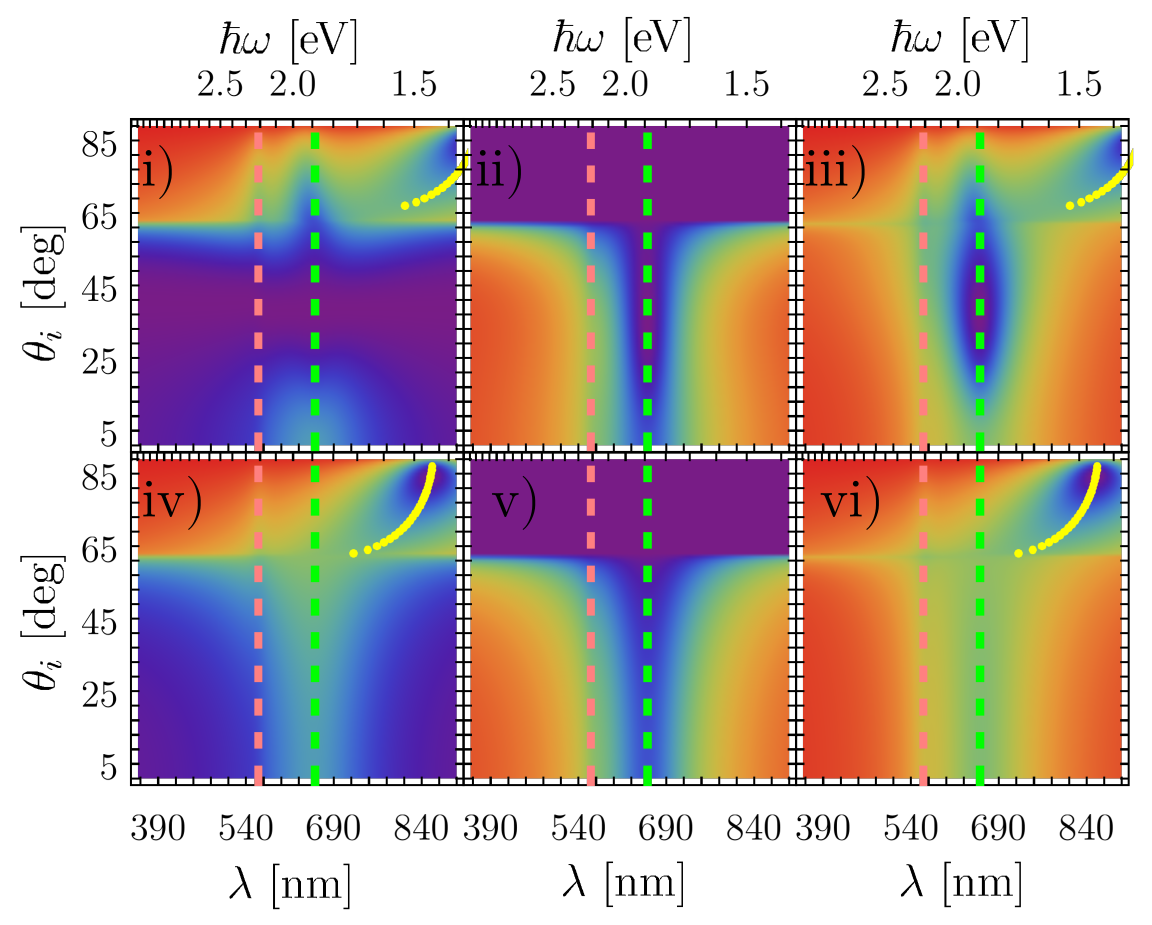
\includegraphics[scale=1]{2-Resultados/figs/5-RT-Wp4-10/0-2D_Grid_1.png}};
\node[right, inner sep=0pt] (legend) at (4.45,.15) {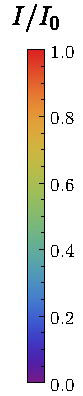
\includegraphics[scale=1, trim={00 -15 00 00}, clip]{2-Resultados/figs/0-IBar_v}};

\def\x{7.5}
	\node at(\x,1){\small $\hbar\omega_p=4.3$ eV};
	\node at(\x,0) {\small $\Theta = 0.2$};
	\node at(\x,-1) {\small $a=30$ nm};

\def\xR{4.2}
\def\yR{.5}	
	\node at(\xR-5.525,\yR){$R_p $};
	\node at(\xR-5.525,\yR-2.8){$R_s$};
		\node at(\xR-2.75,\yR){$T_p $};
		\node at(\xR-2.75,\yR-2.8){$T_s$};
			\node at(\xR-.325,\yR){$R_p+T_p $};
			\node at(\xR-.325,\yR-2.8){$R_s+T_s$};
\end{tikzpicture}	
	\end{subfigure}\\ \noindent \hspace*{-4em}
	\begin{subfigure}{.01\linewidth}\caption{}\label{sfig:RT-10}\vspace{5.5cm}\end{subfigure}\hspace*{-.5em}
	\begin{subfigure}{.7\linewidth}\hspace*{-.5em}
	\begin{tikzpicture}[scale=1]
\node[inner sep=0pt] (graf) at (.05,0){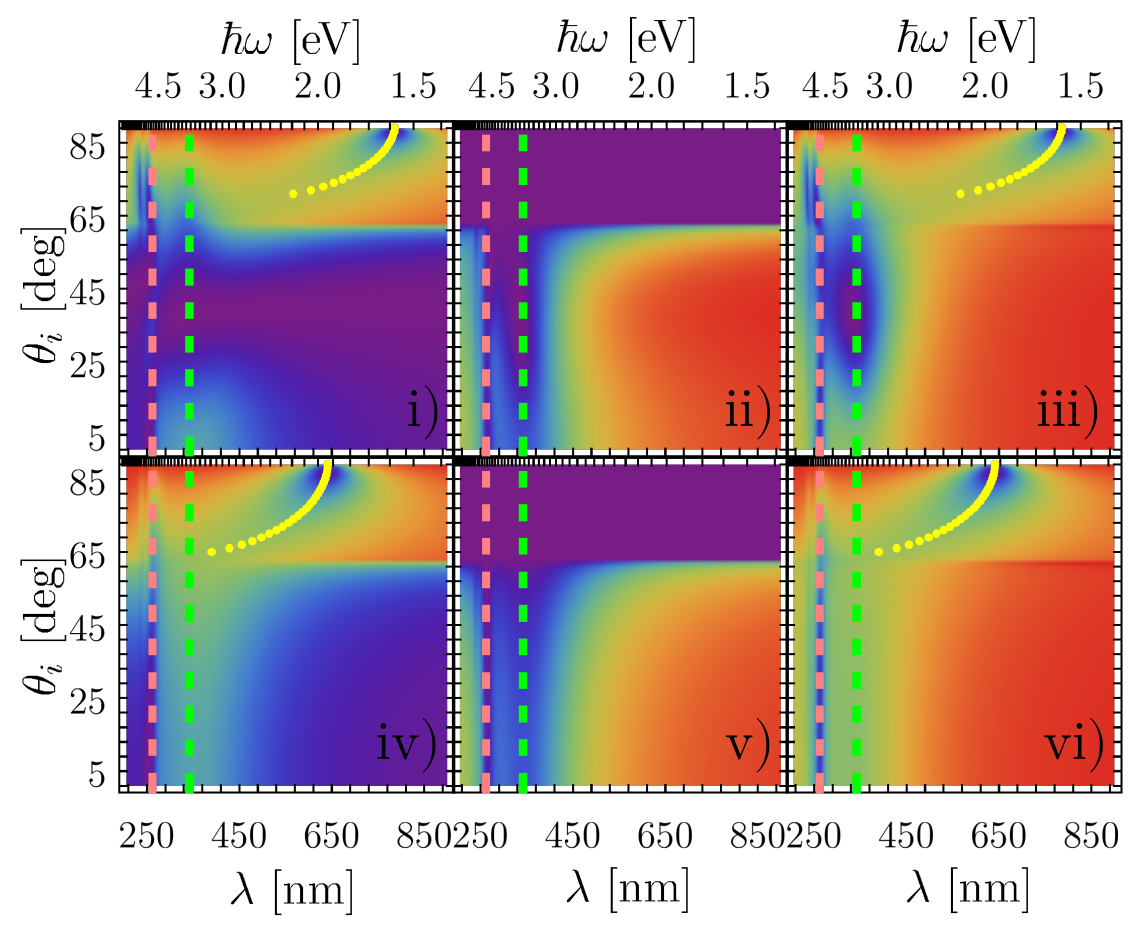
\includegraphics[scale=1]{2-Resultados/figs/5-RT-Wp4-10/0-2D_Grid_2.png}};
\node[right, inner sep=0pt] (legend) at (4.4,.15) {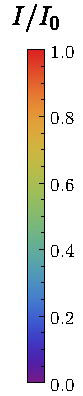
\includegraphics[scale=1, trim={00 -15 00 00}, clip]{2-Resultados/figs/0-IBar_v}};

\def\x{7.5}
	\node at(\x,1){\small $\hbar\omega_p=10$ eV};
	\node at(\x,0) {\small $\Theta = 0.3$};
	\node at(\x,-1) {\small $a=30$ nm};

\def\xR{4.2}
\def\yR{1.}	
	\node at(\xR-5.525,\yR){$R_p $};
	\node at(\xR-5.525,\yR-2.8){$R_s$};
		\node at(\xR-2.75,\yR){$T_p $};
		\node at(\xR-2.75,\yR-2.8){$T_s$};
			\node at(\xR-.325,\yR){$R_p+T_p $};
			\node at(\xR-.325,\yR-2.8){$R_s+T_s$};
\end{tikzpicture}
		\end{subfigure}\vspace*{-.5em}
	\caption{Gráficas de la reflectancia $R$, transmitancia $T$ y su suma $R+T$ en configuración ATR de una monocapa de NPs esféricas como función del ángulo de incidencia $\theta_i$ y de la longitud de onda $\lambda$ (escala inferior) así como de la energía $\hbar\omega$ (escala superior) de la onda plana incidente, considerando NPs con una función dieléctrica tipo Drude con \textbf{a)} $\hbar\omega_p=4. 3$ eV,  $\hbar\gamma=0. 15$ eV y un radio de $a=30$ nm y fracción de cubierta $\Theta=0.2$, y \textbf{b)} $\hbar\omega_p = 10$ eV y $\hbar\gamma = 0.15$ eV con $a=30$ nm y $\Theta=0.3$.  Las gráficas   en el renglón superior [\textbf{i)--iii)}]  muestran los resultados de la reflectancia para  polarización \emph{p} y las del renglón inferior  [\textbf{iv)--vi)}] para polarización  \emph{s}. Las líneas verticales punteadas verdes corresponden a la SP-SPR dipolar ($658$ nm y $342$ nm para $\hbar\omega_p=4.3$ eV y $\hbar\omega_p = 10$ eV, respectivamente), y las rosas a la SP-SPR cuadrupolar ($561$ nm y $262$ nm para $\hbar\omega_p=4.3$ eV y $\hbar\omega_p = 10$ eV, respectivamente). Los puntos amarillos corresponden a los mínimos en $R$, y $R+T$ para ángulos mayores a $\theta_c\approx 62.5^\circ$ y longitudes de onda mayores a la SP-SPRs dipolar. }\label{fig:RT-Omegas}
	\end{figure}	

Para ambos casos analizados en la Fig. \ref{fig:RT-Omegas}, $\hbar\omega_p = 4.3$ eV y $\hbar\omega_p = 10$ eV, se observa que para valores de $\lambda$ cercanos a los de las SP-SPRs (líneas punteadas verticales) la reflectancia $R$ presenta máximos locales para ángulos de incidencia $\theta_i<\theta_c \approx 62.5^\circ$, debido al esparcimiento de luz a esa longitud de onda, y mínimos locales para $\theta_i>\theta_c$, causado por la extinción de luz (tanto esparcimiento como absorción). Por otro lado, la transmitancia $T$ es cercana a cero para todo valor de $\theta_i$ en los valores de $\lambda$ cercanos a los de las SP-SPRs y, adicional a estos valores de $\lambda$, la transmitancia es cero para $\theta_i>\theta_c$, es decir, que a las longitudes de onda que excitan al supuesto modo plasmónico colectivo no hay transmisión de luz. La suma de $R$ y $T$ [en las Figs. \ref{sfig:RT-4} y \ref{sfig:RT-10}, \textbf{iii)} y \textbf{vi)}] en los valores de $\lambda$ que corresponden a las SP-SPRs es menor a la unidad debido a la absorción y esparcimiento de luz por las NPs individuales, como se observa al comparar las eficiencias de extinción para NPs de radio $a=30$ nm inmersa en agua y con una función dieléctrica tipo Drude con los parámetros $\hbar\omega_p=4.3$ eV  y $\hbar\gamma=0.15$ eV [ver  Fig. \ref{fig:QextDrude}]. A pesar de que se pueden presentar procesos de  absorción a longitudes de onda mayores a las de las SP-SPRs (líneas punteadas verticales) debido a la interacción entre las NPs de la monocapa, el supuesto modo plasmónico colectivo se debe al esparcimiento múltiple, lo que propicia que la energía se transporte a lo largo de la interfaz. El resultando de la interacción entre las NPs, además de los procesos de absorción, es el esparcimiento de luz sobre la interfaz, una dirección distinta a la transmitida coherente (es decir $T\approx 0$), por lo que el supuesto modo plasmónico colectivo presenta un comportamiento de modo guiado.

El modelo del CSM predice una excitación colectiva en la respuesta EM de una monocapa de NPs esféricas e idénticas, inmersa en una matriz y soportada por un sustrato al ser iluminada por una onda evanescente, es decir, en una configuración ATR. Esta excitación no corresponde a una SP-SPR pues se excita a energías menores a éstas, y puede catalogarse como un supuesto modo plasmónico colectivo pues depende del radio de las NPs de la moncapa y de su fracción de cubierta, parámetros que modifican la cantidad de electrones libres en la monocapa y cuya elección sintoniza al supuesto modo plasmónico colectivo. Asimismo, este supuesto modo plasmónico colectivo se comporta como un modo guiado pues la suma de la reflectancia y la transmitancia en la dirección coherente de esparcimiento es mucho menor que $1$. Tras la caracterización del supuesto modo plasmónico colectivo, empleando el modelo de Drude-Sommerfeld para la función dieléctrica de las NPs, se analiza si esta excitación colectiva también es apreciable en materiales más realistas. En la siguiente sección se presentan los resultados de la respuesta EM de una monocapa conformada por NPs de oro y plata, es decir, empleando como función dieléctrica de las NPs la corrección por tamaño de los datos experimentales para el oro y plata \cite{johnson1972constants}.

